\documentclass[cn,11pt,twocol]{elegantbook}

\title{程序设计竞赛中的数论}
\subtitle{基础篇}

\author{Yuxiang Chen}
\institute{AHU ACM-ICPC Lab}
\date{\today}
\version{1.0}

\extrainfo{Euclid marched into the wonderful world of Number Theory alone. --- Millay, 1923}

\logo{logo.png}
\cover{cover.jpg}

\usepackage{xcolor}


\colorlet{mygray}{black!30}
\colorlet{mygreen}{green!60!blue}
\colorlet{mymauve}{red!60!blue}

\lstdefinestyle{codestyle2}{
	backgroundcolor=\color{white},  
	basicstyle=\small\ttfamily,
	columns=fullflexible,
	breakatwhitespace=false,      
	breaklines=true,                
	captionpos=b,                    
	commentstyle=\color{mygreen}, 
	extendedchars=true,              
	frame=single,                   
	keepspaces=true,             
	keywordstyle=\color{blue},      
	language=c++,                 
	numbers=left,                
	numbersep=5pt,                   
	numberstyle=\small\color{blue}, 
	rulecolor=\color{mygray},        
	showspaces=false,
	showstringspaces=false,               
	showtabs=false,                 
	stepnumber=1,                  
	stringstyle=\color{mymauve},    
	tabsize=4,                 
	title=\lstname
}

\begin{document}
	
\maketitle

\tableofcontents


\mainmatter
\hypersetup{pageanchor=true}

\chapter*{写在前面}
\addcontentsline{toc}{chapter}{写在前面}
\markboth{Introduction}{}
	参加ACM-ICPC已经快三年了,想着留下些什么,于是决定将数论方面的一些知识整理成册,供后人参考。
	
	这本册子的目的是{\heiti 降低参赛同学们收集数论相关知识的时间成本},对知识点的介绍尽量做到详细且通俗易懂。
	书中会对所有出现的题目提供solution,一些经典的定理、结论还会提供证明。
	
	在册子完成过程中,AHU ICPC-Lab的同学们提出了许多宝贵意见,在此向他们表示衷心的感谢。此外,本书使用了ElegantBook模板
	(\href{https://github.com/ElegantLaTeX/}{https://github.com/ElegantLaTeX/}),减少了许多排版方面的工作,在此也表示感谢!
		
	由于本人水平所限,书中一定存在不少错误,欢迎同学们在GitHub上提出issues或者邮件联系我。\\
	
	\vbox{}
	

联系方式:
	\begin{itemize}
		\item GitHub 网址:\href{https://github.com/Feynman1999/number-theory-tutorial-in-Programming-Competition}{https://github.com/Feynman1999/number-theory-tutorial-in-Programming-Competition}
		\item 邮件:\email{chenyx.cs@gmail.com}
	\end{itemize}

\vbox{}

本书的Tex源码开源在GitHub,未经本人许可不可用于商业用途。\\

\vbox{}

\begin{flushright}
陈昱翔

2019年11月
\end{flushright}
	
\chapter{数的整除性}
\begin{introduction}[本章内容提要]
	\item 欧几里得算法
	\item 拓展欧几里得算法
\end{introduction}

\section{最小公倍数}
两个数a与b(不全为零)的最大公因数是整除它们两个的最大数,记为$gcd(a,b)$。如果$gcd(a,b)=1$,我们称$a$与$b$互质。

求两个数最大公因数的最有效的方法是{\heiti 欧几里得算法},其核心操作是辗转相除,先看一个例子。

\begin{example}
	欧几里得算法求gcd(28,93)的例子。
	
	第一步用93除以28得商为3,余数为7,记作下面式子:
	$$
		93 = 3*28 + 7
	$$
	第二步用上一步的除数作为新的被除数,上一步的余数作为新的除数,即:
	$$
		28 = 4*7 + 0
	$$
	发现此时余数为0,算法不再继续。欧几里得算法指出当得到余数0时,除数(上一步的余数)就是最初两个数的最大公因数。所以
	gcd(28,93) = 7。
\end{example}

\begin{theorem}{欧几里得算法}{label}
	要计算两个整数a与b的GCD,先令$r_{-1}=a$且$r_{0}=b$,然后计算相继的商和余数:$r_{i-1}=q_{i+1}*r_{i}+r_{i+1} \quad (i=0,1,2,...)$,
	直到某余数$r_{n+1}=0$,最后的非零余数$r_{n}$就是a与b的最大公因数。
\end{theorem}

\begin{proof}
	考虑一般情形,有
	\begin{align*}
	r_{-1} &= q_1*r_0 + r_1 \\
	r_0 &= q_2*r_1 + r_2 \\
	r_1 &= q_3 * r_2 + r_3 \\
	r_2 &= q_4 * r_3 + r_4 \\
 	&\cdot \cdot \cdot\\
	r_{n-3} &= q_{n-1}*r_{n-2} + r_{n-1} \\
	r_{n-2} &= q_{n} * r_{n-1} + {\color{red} r_n} \\
	r_{n-1} &= q_{n+1} * r_n + 0 \\
	\end{align*}
	欧几里得算法说,最后的$r_n$就是gcd,那么我们先证明$r_n$一定是$a(r_{-1})$和$b(r_0)$的因子。
	
	由最后一行知,$r_n$整除$r_{n-1}$,于是由倒数第二行知$r_n$整除$r_{n-2}$,依次类推,$r_n$整除$r_{0}$和$r_{-1}$。
	
	下面再证明$r_n$是$a$与$b$的{\heiti 最大}公因数。假设$d$是$a$与$b$的任意公因数,则由上面式子第一行知$d$整除$r_1$,
	于是由第二行知$d$整除$r_2$,依次类推,$d$整除$r_n$,即$r_n$是最大的公因数。
	
	最后,还要说明一定存在$r_{n+1}$为0,易知,每一次余数都是严格递减的,所以余数最后总能到0。那自然会问,要多少步呢?
	实际上,{\heiti 欧几里得算法的步数至多是$b$的位数的7倍}。
\end{proof}


\lstinputlisting[language=C++, style=codestyle2]{code01/gcd.cpp}

说到GCD,往往还会提到最小公倍数(LCM),有如下式子
\begin{align*}
lcm(a,b) * gcd(a,b) &=a*b \\
lcm(S/a, S/b) &= S/gcd(a, b)
\end{align*}


\section{线性方程定理}

已知两个整数a,b,现在我们观察由a的倍数加上b的倍数得到的所有可能整数,也就是说{\heiti 考察$ax+by$得到的所有整数},其中x,y可以是任何整数。

例如取$a=42$,$b=30$,随意列出一些x,y,会发现得到的数都可以被6整除。这其实很显然,因为42和30都能被6整除。更一般的,{\heiti 显然形如$ax+by$的每个数被$gcd(a,b)$整除},因为$gcd(a,b)$整除a与b。

接着问题又来了,$ax+by=gcd(a,b)$是否一定有整数解呢?答案是肯定的。证明是利用{\heiti 拓展欧几里得算法},不停的将余数用a和b表示,{\heiti 最后的gcd(a,b)一定可以用a,b表示}。也称欧几里得回代法。

\begin{example}
欧几里得回代法解$60x+22y=gcd(60,22)$

首先写出欧几里得算法计算gcd(60,22)的过程:
\begin{align*}
60=2 * 22+16 \\
22=1 * 16+6 \\
16=2 * 6+4 \\
6=1 * 4+2 \\
4=2 * 2+0
\end{align*}

这表明gcd=2。下面关键来了,我们想用a,b表示倒数第二行$6=1*4+2$的那个2,就从第一行表示a,b回代,如表\ref{tab:欧几里得回代法示例}:

\begin{table}[!htbp]
	\centering
	\caption{欧几里得回代法示例}
	\begin{tabular}{cccc}
		\toprule
		原式  && & 带入过程  \\
		\midrule
		$a=2*b+16$&&  & $16=a-2*b$ \\
		$b=1*16+6$&& & $6=b-1*16=-a+3b$ \\
		$16=2*6+4$&& &  $4=16-2*6=3a-8b$ \\
		$6=1*4+2$ && & $2=6-1*4=-4a+11b$ \\
		\bottomrule
	\end{tabular}%
	\label{tab:欧几里得回代法示例}
\end{table}%
	
于是得到$x=-4, \ y=11$。

\end{example}

{\heiti 这样一行行进行,将陆续得到形如最新余数=a的倍数+b的倍数的等式,最终得到非零余数gcd,就给出了方程的解。}

\begin{note}
$gcd(a,b)$是否是形如$ax+by$的最小正整数呢?是的。因为$gcd(a,b)<=min(a,b)$。
\end{note}

\vbox{}

既然一个线性方程$ax+by=gcd(a,b)$总有整数解$x,y$,下面的问题是{\heiti 如何表述线性方程的所有解}。

先考虑$gcd(a,b)=1$的情况(即a,b互质,其他情况可以转换为互质),假设$x_1,y_1$是方程$ax+by=1$的一个解。
通过$x_1$加上b的倍数和$y_1$减去a的相同倍数,可得到其他解。即对于任何整数$k$,我们得到新解$(x_{1}+kb,y_{1}-ka)$。(带入即可验证)

\begin{proof}
	$(x_{1}+kb,y_{1}-ka)$可以给出方程的{\heiti 所有}解。
	
	假设$(x_{1},y_{1})$与$(x_{2},y_{2})$是方程ax+by=1的两个解,即$ax_{1}+by_{1}=1$ 且$ ax_{2}+by_{2}=1$ ,我们用$y_{2}$乘以第一个方程,用$y_{1}$乘以第二个方程,再相减消去b,整理后得到$ax_{1}y_{2}-ax_{2}y_{1}=y_{2}-y_{1}$。
	类似的,用$x_{2}$乘以第一个方程,用$x_{1}$乘以第二个方程,再相减便得到$bx_{2}y_{1}-bx_{1}y_{2}=x_{2}-x_{1}$。
	令$k=x_{2}y_{1}-x_{1}y_{2}$,则得到$x_{2}=x_{1}+kb \ ,\  y_{2}=y_{1}-ka$。得证。
\end{proof}

\vbox{}

再考虑$gcd(a,b)>1$的情况,为简便,令$g=gcd(a,b)$,由前面“欧几里得回代法”知方程$ax+by=g$至少有一个解$(x_{1},y_{1})$。
{\heiti 而$g$整除$a,b$},故$(x_{1},y_{1})$是简单方程$\frac{a}{g}x+\frac{b}{g}y=1$的解。
于是由前面证明,通过式子$x_1+k*\frac{b}{g},\ y_1-k*\frac{a}{g}$改变$k$的值可得到其他解。这就完成了对方程ax+by=g解的描述,我们把它概括为下面定理。


\begin{theorem}{线性方程定理}{label}
设$a$与$b$是非零整数,$g=gcd(a,b)$。方程$ax+by=g$总是有一个整数解$(x_{1},y_{1})$(也称贝祖定理),
它可由前面叙述的欧几里得回带法得到。则方程的每一个解可由$(x_{1}+k*\frac{b}{g},y_{1}-k*\frac{a}{g})$得到,其中$k$可为任意整数。
\end{theorem}

\vbox{}

现在我们想怎么用代码实现上面说到的回代法。

如果用上面的思路,我们似乎需要事先知道欧几里得的结果,然后根据结果去算系数。
但是一般用计算机求解gcd,是递归算法,就是说我们需要逆推(上面过程的逆过程),这样才能写出递归代码。

假设当前我们要处理的是求出a 和 b的最大公约数,并要求出 x 和 y 使得 $a * x + b * y=g$。
而我们已经求出了下一个状态:b 和 a\%b 的最大公约数({\heiti 欧几里得算法核心,a=b,b=a\%b}),并且求出了一组$x_1$ 和$y_1$ 使得:$ b * x_1 + (a\%b) * y_1 = g$。
那么这两个相邻的状态之间存在一种关系可以求解,我们知道$a\%b = a - (a/b)*b$,那么较末状态(先开始递归计算的)有:

\begin{align*}
b * x_1 + (a\%b) * y_1 &= g\\
b*x_{1} + (a-(a/b)*b) * y_{1} &= g \\
b*x_{1} + a*y_{1}-(a/b)*b*y_{1} &=g\\
a*y_{1} + b*(x_{1}-a/b*y_{1})&= g
\end{align*}
对比较先的状态(后递归到的,需要求的),需要求一组 x 和 y 使得:$a*x + b*y = g$ ,比较对应项系数得到
\begin{align*}
x &= y_1\\
y &= x_1 - a/b * y_1 \\
\end{align*}


这就是递归的关键,我们把它称为{\heiti 拓展欧几里得算法}。之所以叫拓展,是因为它相比欧几里得算法多了一小点,但能解决模线性方程、逆元、同余方程等许多经典问题(后面会介绍)。

递归的终止条件为$b=0$,这时候$x=1,\ y=0,\ a = gcd$。

\lstinputlisting[language=C++, style=codestyle2]{code01/exgcd.cpp}

\vbox{}

\begin{problemset}
	\item 拓展欧几里得算法的时间复杂度是多少?
	\item \href{http://poj.org/problem?id=1061}{青蛙的约会}
	\item \href{https://ac.nowcoder.com/acm/contest/201/C}{Utawarerumono}
\end{problemset}











\chapter{素数}
\begin{introduction}[本章内容提要]
	\item 质因数分解
	\item 筛选素数
	\item 大区间问题
	\item 梅森素数
	\item 完全数
	\item 因数之和函数
\end{introduction}

\section{质因数分解}
\begin{definition}{素数}{prime}
	素数$p$是大于1且它的因数只有1和$p$的整数。
\end{definition}

\begin{property}
	\label{pro:prime}
	令p是素数,假设p整除乘积ab,则p整除a或p整除b(或者p既整除a也整除b)  
\end{property}

\begin{theorem}{无穷多素数定理}{label}
	存在无穷多个素数。
\end{theorem}

\begin{proof}
	证明的思路是,假设我们现在有一个素数表,只要说明如何利用这些素数找出新的不在表中的素数,这样迭代下去,就
表明必有无穷多个素数。设素数表一开始为$p_1,p_2,...,p_n$,令$A = p_1p_2...p_n + 1$,设$q$是某个整除$A$的素数,且设其是
最小的那个,那么$q$一定不在最初的素数表中,因为如果$q=p_i$,则$q$能整除1,显然错误。于是我们可以无限扩充素数表。
\end{proof}

\begin{theorem}{素数定理}{label}
	当x很大时,小于x的素数的个数近似等于$x/ln(x)$,即
	$$
	\lim_{x\to\infty} \frac{\pi(x)}{x/ln(x)}=1
	$$
	其中$\pi(x)$为素数计数函数,$\pi(x) = \#\{prime\ p:p\le x\}$。
\end{theorem}

\begin{theorem}{素数整除性质}{label}
假设素数p整除乘积$a_1a_2...a_r$ ,则p整除$a_1 \quad ,a_2 \quad , ...,\quad a_r$ 中至少一个因数。
\end{theorem}

\begin{proof}
	使用上面的\hyperref[pro:prime]{性质}可以方便的证明该定理。
\end{proof}

\vbox{}

下面将用{\heiti 素数整除性质}证明每个正整数可唯一分解成素数的乘积(算术基本定理)。

\begin{theorem}{算术基本定理}{suanshu}
	每个整数n>=2可唯一分解成素数乘积$n=p_1p_2...p_r$。
\end{theorem}

\begin{proof}
算术基本定理包含两个断言:

断言1:数n可以以某种方式分解成素数的乘积;

断言2:仅有一种这样的因数分解方式(因数重排除外);

- 对于断言1的证明用到归纳证明法 (当N+1是合数时,其必然可以分解成$N+1=n_1*n_2$,而前面已经归纳完毕,即$n1,\ n2$一定可以分解成素数,因此得证)。

- 对于断言2,可以由定理\ref{thm:suanshu}证得。
\end{proof}

\vbox{}

下面考虑如何进行质因数分解。

简单直接的方法是试除2,3,4,5,...分解n,但效率较低。
考虑一个整数n,如果n本身不是素数,则必有整除n的素数$p\leqslant \sqrt{n}$ 。于是我们可以遍历$2\sim \sqrt{n}$
进行试除,时间复杂度为$O(\sqrt{n})$。如果提前预处理出所有素数,则可每次只试除素数,时间复杂度为$O(\frac{\sqrt{n}}{ln \sqrt{n}})$

\lstinputlisting[language=C++, style=codestyle2]{code02/factor.cpp}

\section{区间素数筛}

这里区间素数筛指的是给定一个上限$n$,要求出区间$[1,n]$中所有的素数。如果采用直接遍历每个数并判断是不是素数的方法,时间复杂度为$O(n^{3\over2})$,若$n>10^6$,则
不能在$1s$的时间内求解。下面介绍的两种筛法,均使用“筛选”的思想,时间复杂度分别为$O(nlog(logn))$和$O(n)$,在比赛中经常使用。

\subsection{埃氏筛法}
考虑如果一个数$n$如果是合数(非素数),那么它一定有小于等于$\sqrt{n}$的质因子,也即$n$是这个质因子的倍数。那么我们可以从小到大($2\sim n$)依次遍历每个数,并存在一些标记记录每个数是否是合数,当遍历到某个数
时,如果当前数没有被标记为合数(就一定是素数了),就把当前数的所有倍数标记为合数。代码如下:

\lstinputlisting[language=C++, style=codestyle2]{code02/aishi.cpp}

\begin{remark}
	代码中有两个关键的地方:
\begin{itemize}
	\item 第10行,只有当是素数时,才进行筛选,因为使用合数筛是多余的(该合数的质因子已经筛过了);
	\item 第12行,从$i*i$开始筛,因为$(i-1)*i,\ (i-2)*i,\ ...\ 2*i$已经被筛过了。
\end{itemize}
\end{remark}

考虑埃氏筛法的时间复杂度,由于每次只考虑素数去筛,即为:
$$
	n\sum_{p\le n} \frac{1}{p}\ , \quad p \ is \ prime
$$
上式可近似认为是$O(nloglogn)$,感兴趣的可以阅读\href{http://www.wikiwand.com/en/Sieve_of_Eratosthenes#/Algorithm_complexity}{Sieve\_of\_Eratosthenes\#/Algorithm\_complexity} 

\vbox{}

观察埃氏筛法,是否有重复被筛去的合数呢?有的,就是一些质数的较大的公倍数,比如12,当i=2时(从4开始)会筛12;当i=3时(从9开始)还会筛12。

\subsection{欧拉线性筛法}

	欧拉筛的思想是{\heiti 保证每个合数都被其最小的质因子筛去},这样就不会像埃氏筛那样重复筛某个数。

	首先其还是筛选法,考虑用什么筛的:对于每个i,乘以小于i的每个素数,直到能整除就停止,这样能保证每个数只被筛去一次。
	
	这个整除停止很关键,假设没有这个break,就会有很多重复。
	
	比如$i=6$,取质数3,筛去了18;$i=9$,取质数2,也筛去了18。
	
	再比如$i=6$,取质数5,筛去了30;$i=10$,取质数3,筛去了30;$i=15$,取质数2,筛去了30。
	
	如果加上break,则筛去18的是9*2,筛去30的是15*2。为什么18不会被6*3筛去? 因为$6\%2=0$
	提前break了。即若有一个素数$p|i$,则我用i和后面更大的素数去筛选,不如用p和更大的i去筛选,
	这样保证了筛掉每个数的是其最小质因子。
	
	
\lstinputlisting[language=C++, style=codestyle2]{code02/euler.cpp}

由于每个数只会被筛去一次,时间复杂度是$O(n)$。

\subsection{区间数的最大、最小质因子}
上面介绍的埃氏筛法和欧拉筛法经过一点改动就可以用来求区间数的最大质因子和最小质因子。

对于区间最大质因子,稍微增加点埃氏筛的复杂度,从$2*i$而不是$i*i$开始筛:

\lstinputlisting[language=C++, style=codestyle2]{code02/maxprime.cpp}

对于区间最小质因子,只需修改欧拉筛中标记数组即可,时间复杂度不变:

\lstinputlisting[language=C++, style=codestyle2]{code02/minprime.cpp}


\section{区间质因数分解}
这里区间质因数分解指的是给定一个上限$n$,要求出区间$[1,n]$中所有数质因数分解的结果。
可以用埃氏法先求出所有数的所有质因子;或者使用欧拉法求出区间数的最小质因子再利用区间信息求解。
\subsection{埃氏法}
先$O(nlogn)$求出每个数的所有质因子,再$O(nlogn)$直接除求出质因子对应的指数:

\lstinputlisting[language=C++, style=codestyle2]{code02/interaishi.cpp}

\subsection{欧拉法}
先$O(n)$欧拉筛求出每个数的{\heiti 最小质因子},再$O(nlogn)$利用区间信息求出对应的指数。
区间信息指的是,对于每个数如果我们都知道其最小质因子,则可以先将当前数的最小质因子除完,剩下的数的最小质因子我们还是知道的,于是继续除,直到1为止。
\lstinputlisting[language=C++, style=codestyle2]{code02/intereuler.cpp}

\section{大区间素数筛与质因数分解}
大区间指的是咱们考虑的区间不再是$[1,n]$,而是$[L,R]$,这里$R\le 2^{40}, \  R-L<=10^6$。

\subsection{大区间素数筛}
对于一个合数$n$,一定有小于等于$\sqrt{n}$的质因子,利用这一点,我们依然可以使用埃氏筛的思想。
先预处理出$[1,\sqrt{R}]$区间内的所有素数,然后拿这些素数去做筛选即可。

时间复杂度为$O(N + llogl)$ , 其中$N$为$\sqrt{R}$,$R$是区间右端点,即需要预处理的素数范围 ; $l$为区间长度$R-L$。

\lstinputlisting[language=C++, style=codestyle2]{code02/large-inter-prime.cpp}

\subsection{大区间质因数分解}
和上面类似,先埃筛求出小于等于$\sqrt{R}$的所有质因子,然后对于区间内的每个数直接除即可。

因为一个合数n大于$\sqrt{n}$ 的质因子最多只有1个,因此将已知的质因子全部除尽后,若不为1,就为那个大于$\sqrt{n}$的质因子,对应指数为1。

时间复杂度为$O(N + llogl)$,其中$N$为$\sqrt{R}$,$R$是区间右端点,即需要预处理的素数范围 ; $l$为区间长度$R-L$。

\lstinputlisting[language=C++, style=codestyle2]{code02/large-inter-factor.cpp}


\section{梅森素数与完全数}
梅森素数与完全数在程序设计竞赛中不是很常见,这里简要介绍一下。

\subsection{梅森素数}
现在我们来研究形如$a^n-1(n\ge2)$的素数。例如31就是这样的数,因为$31 = 2^5 - 1$。
由于$a-1$始终是$a^n-1$的因子。为啥呢?因为使用几何级求和公式:(展开即可证明该公式)
$$
x^n-1=(x-1)(x^{n-1}+x^{n-2}+...+x^2+x+1)
$$
所以若$a^n-1$为素数,则a一定等于2。反之显然不成立。

再进一步考虑$n$,假设$n$为合数,即$n=mk$,则$2^n=2^{mk}=(2^m)^k$。使用$x=2^m$的几何级数公式得:
$$
2^n - 1 = (2^m)^k - 1 = (2^m-1)((2^m)^{k-1}+(2^m)^{k-2}+...+(2^m)^2+(2^m)+1)
$$
这证明了若$n$是合数,则$2^n-1$也是合数。综上有以下命题:

\begin{proposition}{}{label}
	如果对整数$a\ge2$与$n\ge2$,$a^n-1$是素数,则$a$必等于2且$n$一定是素数。
\end{proposition}

形如$2^p-1$的素数叫做{\heiti 梅森素数},已知的梅森素数在\href{https://www.mersenne.org/primes/}{https://www.mersenne.org/primes/}中可以找到,
目前已经找到了51个(截至2019.09.03)。发现更多的梅森素数没有太大的数学意义,数学上更令人感兴趣的是下面的问题,其答案尚未知晓:

\begin{custom}{问题}
	存在无穷多个梅森素数吗?
\end{custom}

\subsection{完全数}

\begin{definition}{完全数}{wanquanshu}
	完全数是等于其真因数之和的数。真因数指的是小于自己的因数(即除去自己)。
\end{definition}


\begin{theorem}{欧几里得完全数公式}{label}
	如果$2^p-1$是素数,则$2^{p-1}(2^p-1)$是完全数。
\end{theorem}

\begin{proof}
	将$2^{p-1}(2^p-1)$所有真因数直接写出求和即证。
\end{proof}

这里的$(2^p-1)$不就是梅森素数吗?也就是说只要求得一个梅森素数,就得到一个完全数。

那欧几里得完全数公式是否表示了所有完全数呢?千年之后的欧拉证明了欧几里得完全数公式至少给出了所有{\heiti 偶完全数},称为欧拉完全数定理。

在介绍和证明欧拉完全数定理之前,我们先来介绍一个函数$\sigma(n)$。

\begin{center}
	$\sigma(n) = n$的所有因数之和(包括1和n)。
\end{center}

例如$\sigma(6) = 1 + 2+3+6 = 12$。下面试着写出其一般公式,$\sigma(p) = p+1$,$\sigma(p^k) = 1 + p+p^2+...+p^k = \frac{p^{k+1}-1}{p-1}$。

如果你用程序打个表,也许会发现$\sigma(mn)$时常会等于$\sigma(m)\sigma(n)$,实际上这在$m$和$n$互质时成立。

\begin{theorem}{$\sigma$函数公式}{label}
	\begin{itemize}
		\item 如果$p$是素数,$k\ge1$,则$\sigma(p^k) = 1 + p+p^2+...+p^k = \frac{p^{k+1}-1}{p-1}$;
		\item 如果$gcd(m,n)=1$,则$\sigma(mn) = \sigma(m)\sigma(n)$。
	\end{itemize} 
\end{theorem}

$\sigma$函数在程序设计竞赛中也时常出现(或者其类似函数,如因子个数函数),后面章节还会说到它,现在我们用它来辅助证明欧拉完全数定理。

显然,$\sigma$函数可以和完全数产生联系,如果$\sigma(n)=2n$,则n恰好是完全数。

\begin{theorem}{欧拉完全数定理}{label}
如果n是偶完全数,则$n$一定是$2^{p-1}(2^p-1)$ 的形式,其中$2^p-1$是梅森素数。
\end{theorem}

\begin{proof}
	假设n是偶完全数,n是偶数则说明可将它分解成$n=2^km,\quad k\ge 1 \ \&\ m\ is\ odd$
	
	则$\sigma(n)=\sigma(2^km)=\sigma(2^k)\sigma(m)=(2^{k+1}-1)\sigma(m)$。
	又n是完全数,则$\sigma(n)=2n=2^{k+1}m$。
	
	因此可以得到
	$$
	2^{k+1}m=(2^{k+1}-1)\sigma(m)
	$$
	由上式可知,由于$(2^{k+1}-1)$一定是奇数,所以$2^{k+1}| \sigma(m)$ ,于是设$\sigma(m)=c*2^{k+1}$ ,带入上式有:
	\begin{align*}
	2^{k+1}m=(2^{k+1}-1)*c*2^{k+1} \\
	m=(2^{k+1}-1)*c
	\end{align*}
	现在我们有两个式子,$m=(2^{k+1}-1)*c$ 和$\sigma(m)=c*2^{k+1}$。
	
	实际上这里c只能等于1,下面我们来证明$c=1$。
	
	假设$c>1$,则$m=(2^{k+1}-1)*c$至少被不同的数$1,c,m$所整除,因此有
	$$
	\sigma(m)\ge 1+c+m=1+c+(2^{k+1}-1)*c
	$$
	显然,这是错误的(会得出$0\ge 1$),因此$c=1$,所以$m=2^{k+1}-1$  ,  $\sigma(m)=2^{k+1}=m+1$,所以m是素数。
	
	现在我们已经证明了,如果n是偶完全数,则
	$$
	n=2^k(2^{k+1}-1)\ ,\quad where \ (2^{k+1}-1)\ is \ prime
	$$
	由于$2^{k+1}-1$是素数,则$(k+1)$一定是素数,(上节已说明)。令$k+1=p$,则$n=2^{p-1}(2^p-1)$,其中$2^p-1$是梅森素数。
	
	欧拉完全数定理证毕。
\end{proof}

\vbox{}

\begin{note}
	关于完全数的几个结论:
	\begin{itemize}
		\item 目前还没找到奇完全数
		\item 每个完全数的全部因数倒数之和都是2
		\item 除了6以外的完全数,每个都可以表示成连续奇数的立方和
		\item 每个完全数都可以表示成2的一些连续正整数次幂之和
		\item 完全数都是以6、8结尾
	\end{itemize}
\end{note}

\vbox{}

\begin{custom}{问题}
	存在奇完全数吗?
\end{custom}

\vbox{}

\vbox{}


\begin{problemset}
	\item 区间数的最大质因子是否有线性时间的算法?
	\item 大区间数的最小质因子是否有线性时间的算法?
	\item 试着写出求单点$\sigma(n)$以及区间$[1,n]$所有$\sigma$值的代码。
\end{problemset}
\chapter{同余}

\begin{introduction}
\item 同余方程
\item 快速乘、快速幂
\item 逆元、线性求区间逆元
\item 中国剩余定理
\item 欧拉降幂
\item 卡米歇尔数
\item Miller\_Rabin
\item Pollard\_Rho
\item 离散对数
\item 原根
\end{introduction}


\section{同余式与同余方程}
\subsection{同余式}
整除性是很好的性质,这在最大公因数、模线性方程和素数分解中均得到了体现。而同余式提供了一种
描述整除性质的简便方式。

\begin{definition}{同余}{label}
	如果$m|(a-b)$,我们就说a与b模m同余并记之为$a\equiv b(mod\ m)$。
	
	特别地,$a\equiv a\%m(mod\ m)$ 。
\end{definition}

数m叫做同余式的模。 具有相同模的同余式在许多方面表现得很像通常的等式。例如:

若$a_1\equiv b_1(mod\ m) \ ,\quad a_2\equiv b_2(mod\ m)$     则$a_1\pm a_2\equiv b_1\pm b_2(mod \ m)$ ,$a_1a_2\equiv b_1b_2(mod \ m)$ 

{\heiti 但 $ac\equiv bc(mod \ m)$ 时,未必有$a\equiv b(mod \ m)$,只有$gcd(c,m)=1$,才可以消去c。}


\subsection{同余方程}
如果同余式含有未知数,我们考虑如何求解。

首先考虑“穷举法” ,要解模m同余式,可让每个变量试取0,1,2...,m-1。例如,解同余式$x^2+2x-1\equiv 0(mod\ 7)$,
就去试$x=0\quad, x=1\quad,...\quad,x=6$,这样可以求出两个解$x\equiv 2(mod\ 7)$和$x\equiv 3(mod\ 7)$ 当然还有其他解,但新的解与2或3是同余的,如9和10。当我们说“求同余式的所有解时”,是指求所有不同余的解,即相互不同余的所有解。

许多同余式是没有解的,如$x^2\equiv 3(mod\ 10)$。

\vbox{}

下面考虑如何求解同余式$ax\equiv c(mod\ m)$。 
\begin{example}
解同余式$18x\equiv8(mod\ 22)$
\end{example}

等价于求$22\ |\ (18x-8)$,即求$18x-22y=8$。       

解这类方程的问题在第一章中研究过。

对于$ax\equiv c(mod\ m)$ ,其有解{\heiti 当且仅当}线性方程$ax-my=c$ 有解。


由前可知,线性方程$ax-my=c$ 有解的充分必要条件是$gcd(a,m)\ |\ c$。

且方程$au+mv=g$ 一定有解 ,设一个解为$(u_0,v_0)$,则有
$$
a\frac{cu_0}{g}+m\frac{cv_0}{g}=c
$$
这说明$x_0= \frac{cu_0}{g}$是同余式$ax\equiv c(mod\ m)$ 的一个解,通解为$x=x_0+k\cdot \frac{m}{g}$。

{\heiti 由于相差m的倍数的任何两个解认为是相同的},所有恰好有$g$个不同的解,这些解通过取$k=0,1,2...,g-1$而得到。将上述过程概述为定理:


\begin{theorem}{线性同余式定理$ax\equiv c(mod\ m)$}{label}
设a,c与m是整数,m>=1,且设$g=gcd(a,m)$。 

(a)  如果$g\nmid c$,则同余式$ax\equiv c(mod\ m)$ 没有解

(b)  如果$g\ |\ c$ ,则同余式$ax\equiv c(mod\ m)$ 恰好有g个不同的解。要求这些解,首先求线性方程$au+mv=g$ 的一个解$(u_0,v_0)$ 
{\heiti (欧几里得回带法,在计算机上递归求得,称为扩展欧几里得算法)} 。则$x_0=(\frac{cu_0}{g}\% \frac{m}{g} + \frac{m}{g}) \% \frac{m}{g}$是$ax\equiv c(mod\ m)$ 的解,不同余解的完全集由
$$
x\equiv x_0+k\cdot \frac{m}{g} \  (mod\ m),\quad k=0,1,2,...,g-1
$$
给出。
\end{theorem}


例如,同余式$943x\equiv 381(mod\ 2576)$ 无解,这是因为$gcd(943,2576) \nmid 381$。

另一方面,同余式$893x\equiv 266(mod\ 2432) $
有19个解,因为$gcd(893,2432)=19,\  19|266$     这个19即为不同余解的个数。

下面解方程$893u-2432v=19$ ,使用欧几里得回带法可以求得解$(u,v)=(79,29)$ ,乘以266/19=14得方程$893x-2432y=266$的解$(x,y)=(1106,406)$ ,
即1106是同余式方程的一个解,这样的互不同余的解共有19个。1106加上2432/19=128的倍数(\%2432)就可得到完全解集。


\begin{remark}
	线性同余式定理最重要的情形是$gcd(a,m)=1$ ,在这种情形下,同余式恰好有一个解。
\end{remark}

\lstinputlisting[language=C++, style=codestyle2]{code03/modequation.cpp}

\vbox{}

对于非线性的同余式,其解“不是很确定”。

我们熟悉的是对于{\heiti 一个d次实系数多项式的实根不超过d个} ,这个结论对于同余式并不成立。

例如$x^2+x\equiv 0(mod\ 6)$ 有4个模6不同的根:0,2,3,5。

但是,{\heiti 当p为素数时,这个结论依然成立:}

\begin{theorem}{模p多项式根定理}{label}
设p为素数,$f(x)=a_0x^d+a_1x^{d-1}+...+a_d$ 是次数为d>=1的整系数多项式,且p不整除$a_0$ ,则同余式$f(x)\equiv 0(mod\ p)$ 最多有d个模p不同余的解。
\end{theorem}

\section{快速乘与快速幂}
快速乘和快速幂作为工具经常在程序设计竞赛中遇见。
\subsection{快速乘}
在$C++$中,变量最多只能表示到$2^{64}-1$这么大,所以如果我们要计算$a*b\%c$,而$a,b$都是接近表示上限的数,这个时候就需要快速乘。
即将$b$按二进制位分解分别加上,时间复杂度为$O(log(b))$。
\lstinputlisting[language=C++, style=codestyle2]{code03/fastmul.cpp}

\subsection{$O(1)$快速乘}
上面的“快速乘”时间是$O(logb)$的,如果是两个63位数相乘(结果long long 存不下),则还有一个巧妙的方法可以简单解决这个问题:

\lstinputlisting[language=C++, style=codestyle2]{code03/o1fastmul.cpp}

首先使用浮点运算来得到$\left\lfloor\frac{a * b}{P}\right\rfloor$的值,显然$a*b-d*p$中的两个乘法都有可能会溢出,但是没关系,因为可以知道其差是一个64bit可容纳的正整数,那么溢出部分的差仅可能为0或者1,最后
特判处理一下即可。	
\begin{note}
	当然,如果编译器支持$int128$的话,可以直接用128位数。
\end{note}

\subsection{快速幂}
现在我们要计算$a^b\%c$,如果乘$b$次,时间复杂度太高,考虑将$b$按照二进制分解,每一位分别计算并乘在一起即可。
时间复杂度为$O(log(b))$。相比于快速乘,只是加法变了乘法。
\lstinputlisting[language=C++, style=codestyle2]{code03/fastexp.cpp}


\section{费马小定理与逆元}
前面我们讨论了关于同余式、同余方程的一些性质,小结一下,互质这个条件很重要。

\begin{itemize}
	\item 对于$ac\equiv bc(mod \ m)$,如果$gcd(c,m)=1$,则可以消去c,得到$a\equiv b(mod \ m)$ 。
	\item 对于同余方程 $ax\equiv c(mod\ m)$,若$gcd(a,m)=1$ ,同余式恰好有一个解。
\end{itemize}

{\heiti 对于式子$ax\equiv c(mod\ m)$,令$c=1$,得$ax\equiv 1(mod\ m)$,若$gcd(a,m)=1$,则方程有唯一解$x_0$,
我们称$x_0$为$a$在模$m$意义下的逆元,常记作$a^{-1}$。}

逆元可以用来说明一些事情,比如如果$ac\equiv bc(mod\ m)$,若$gcd(c,m)=1$,
则存在$c^{-1}$使得$cc^{-1}\equiv 1 (mod\ m)$。所以可以对$ac\equiv bc(mod\ m)$两边同时乘以$c^{-1}$,得到$a\equiv b(mod\ m)$。

如何求解逆元呢?拓展欧几里得即可,因为就是一个同余方程:
\lstinputlisting[language=C++, style=codestyle2]{code03/inverse.cpp}

\vbox{}

若模数是素数,我们还可以用费马小定理求解。

\begin{theorem}{费马小定理}{femat}
	设p是素数,a是任意整数且$p\nmid a$ ,则 $a^{p-1}\equiv 1(mod\ p)$。 
\end{theorem}

在证明费马小定理之前,先来看一个引理。

\begin{lemma}{为证明费马小定理做准备}{forfemat}
	设$p$是素数,a是任何整数且 $p\nmid a$ 则数
	$$
	a,2a,3a,...,(p-1)a\qquad (modp)
	$$
	与数
	$$
	1,2,3,...,(p-1)\qquad (modp)
	$$
	相同,尽管它们的次序不同。
\end{lemma}

\begin{proof}
	数列$a,2a,3a,...,(p-1)a$,包含$p-1$个数,显然没有一个数被$p$整除 ,假设从中取出两个数ja和ka是关于p同余的,即$p|(j-k)a$,
	又p是素数且p不整除a,所以p整除$(j-k)$。但是$|j-k|<p-1 $,所以$j-k=0$,即$j=k$。
	
	这表明,这p-1个数模p不同,由于任何数mod p仅有$p-1$个不同的非零值,证毕。
\end{proof}

\begin{proof}
	费马小定理的证明。
	
	利用该引理\ref{lem:forfemat},即可完成对费马小定理\ref{thm:femat}的证明,将上面引理列到的两组数相乘,可得到
	$$
	a^{p-1} \cdot (p-1)!\equiv (p-1)!   \qquad (modp)
	$$
	由于$(p-1)!$与p互质(显然除了1没有其它公共因子了),可以消去它(本节开头有提到这个性质),则$a^{p-1}\equiv 1(mod\ p)$。
\end{proof}

\vbox{}

有了费马小定理,若模数$m$是质数,则数$a$关于$m$的逆元就是$a^{m-2}$,因为$a* a^{m-2} \equiv 1 \ (mod p)$。
使用快速幂直接计算即可。

\vbox{}

{\heiti 使用费马小定理还可以进行素数测试},后面小节会提到。

\section{中国剩余定理}

\begin{theorem}{中国剩余定理}{CRT}
	设m与n是整数,$gcd(m,n)=1$,b与c是任意整数,则同余式组
	$x\equiv b(mod\ m)$与$x\equiv c(mod\ n)$恰有一个解$0\leqslant x<mn$。
\end{theorem}

\begin{proof}
	对于第一个同余式$x\equiv b(mod\ m)$,其解由形如$x = my +b$的所有数组成。将其带入第二个方程可得
	$my\equiv c-b (mod\ n)$,已知$gcd(m,n)=1$,由线性同余式定理知其恰有一个解$y_1,\ 0\le y_1<n$,则$x_1=my_1+b$
	给出了原来同余式组的解,这是在$[0,mn)$之间的唯一解。
\end{proof}

\vbox{}

上面只考虑了两个同余式,如果有多个呢?

\begin{custom}{问题}
	求出方程组$x\equiv a_i(mod \ m_i) (0 \leqslant i <n) $ 的解$x$,其中$m_0,m_1,m_2,m_3,...,m_{n-1}$ 两两互质。
\end{custom}

\begin{solution}
	令$M_i=\prod_{j\neq i}m_j$     则有$(M_i,m_i)=1$   
	
	故存在$p_i,q_i$ ,使得$M_i*p_i+m_i*q_i=1$ 
	
	令  $e_i=M_ip_i$,\quad    $p_i$即为$M_i$ 模$m_i$下的逆元。   
	
	则有
$$
e_i\equiv\left\{\begin{matrix}
0(mod\ m_j)\ ,\ j\neq i\\ 
1(mod\ m_j)\ ,\ j=i
\end{matrix}\right.	
$$	
	故$e_0a_0+e_1a_1+e_2a_2+...+e_{n-1}a_{n-1}$是方程的一个解。
	
	由中国剩余定理知,$[0\sim\prod_{i=0}^{n-1}m_i\}$ 中必有一解,将上式模$\prod_{i=0}^{n-1}m_i$即可。 
\end{solution}

时间复杂度  $O(nlogm)$,其中$n$表示有$n$个方程。

\lstinputlisting[language=C++, style=codestyle2]{code03/crt.cpp}

\begin{custom}{问题}
	如果这些方程的{\heiti 模数不互质}呢?(上面互质的方法只是一种巧妙的构造)
\end{custom}

一样可以求解,每一次我们将两个方程合并为一个方程,具体来说,假设目前的前两个方程为$x\equiv a_1 \ (mod\ m_1),\quad  x\equiv a_2 \ (mod\ m_2)$。
将第一个带入第二个可得到$km_1\equiv a_2-a_1 \ (mod\ m_2)$,解这个同余方程,求出$k$的最小正整数解$k_0$,那么$k = \frac{m_2}{gcd}y+ k_0$,带入
$x=km_1+a_1$中可以得到$x=\frac{m_1m_2}{gcd}y+m_1k_0+a_1$,也即将前两个方程合并为了一个:$x\equiv m_1k_0+a_1\ (mod\ \frac{m_1m_2}{gcd})$,
这样迭代下去,最后的那个方程即为所求。

时间复杂度为$nlogm$,其中$n$是方程个数。{\heiti 代码中的$x_0$即为上面的$k_0$。}

\lstinputlisting[language=C++, style=codestyle2]{code03/excrt.cpp}

\section{欧拉公式与欧拉降幂}

\subsection{欧拉公式}

费马小定理很漂亮$a^{p-1}\equiv 1(mod\ p)$,但限制$p$是素数且$p\nmid a$。如果$p$是合数,即使$a,p$互质,结论也不正确了。
那是否有$a^{???}\equiv 1(mod\ m)$成立的指数呢?带规律的那种。
首先,如果a的某个幂模m余1,则a和m必互质(可由线性方程定理证明)。

这再次提醒我们观察与m互素的数的集合:
$$
{a:1\leqslant a\leqslant m,\quad gcd(a,m)=1}
$$
{\heiti 在1$\sim$m之间与m互质的整数个数}是个重要的量,我们赋予这个量一个名称:


\begin{definition}{欧拉函数$\varphi$}{label}
$$
\varphi(m)=\{a:1\leqslant a\leqslant m,\quad gcd(a,m)=1\}
$$
\end{definition}

注意p是素数时,每个整数$1\leqslant a<p$ 都与p互素,所以对于素数p有公式
$$
\varphi(p)=p-1
$$
我们设法模仿费马小定理的证明。例如,假设要求7的幂次模10余1,不取所有1$\sim$9,而是恰好取与10互素的数,它们是
$$
1,3,7,9
$$
如果用7去乘每个数可得
$$
7\cdot 1\equiv 7(mod\ 10)\quad 7\cdot 3\equiv 1(mod\ 10)\quad
7\cdot 7\equiv 9(mod\ 10)\quad 7\cdot9\equiv 3(mod\ 10)
$$
{\heiti 得到的4个数是之前的4个数的重排!}如果将它们乘起来就得到相同的乘积
\begin{align*}
(7\cdot 1)(7\cdot 3)(7\cdot7)(7\cdot9)\equiv 1\cdot3\cdot7\cdot9  \qquad  (mod\ 10)  \\
7^4(1\cdot3\cdot7\cdot9)\equiv 1\cdot3\cdot7\cdot9 \qquad (mod\ 10)
\end{align*}

由于$1\cdot3\cdot7\cdot9$与$10$是互质的,因此可以消去,所以得到$7^4\equiv 1(mod\ 10)$,这个形式和费马小定理很像了!

考虑这里的指数4和费马小定理中的$p-1$的共同点, 都是1$\sim$m中与m互质的数的个数,即欧拉函数$\varphi(m)$。


\begin{theorem}{欧拉公式}{eulerf}
如果$gcd(a,m)=1$ ,则
$$
a^{\varphi(m)}\equiv 1 (mod\ m)
$$
\end{theorem}

\begin{lemma}{为证明欧拉公式做准备}{foreulerf}
如果$gcd(a,m)=1$,则数列
$$
b_1a,\ b_2a,\ b_3a,\ ...\ ,b_{\varphi(m)}a  \qquad  (mod\ m)
$$
与数列
$$
b_1,\ b_2,\ b_3,\ ...\ ,b_{\varphi(m)} \qquad (mod\ m)
$$
相同,尽管它们可能次序不同,$b_i$表示小于$m$且与$m$互质的数。
\end{lemma}

\begin{proof}
引理的证明。
\begin{itemize}
	\item 注意到$b_i$和a均与m是互质的,则$b_ia$也与m互质。{\heiti 又因为所有与m互质的数\%m后依然与m互质} 
	(如果x-km与m不互质,则x与m也不互质了),所以数列$b_1a,b_2a,b_3a,...,b_{\varphi(m)}a  \quad  (mod\ m)$ 同
	余于数列$b_1,b_2,b_3,...,b_{\varphi(m)} \quad (mod\ m)$ 中的某一个数(因为就这$\varphi(m)$个和$m$互质)。又
	每个数列有$\varphi(m)$个数 ,因此,如果能进一步证明第一个数列中的数对于模m互不相同,就可得出两个数列(重排后)
	相同。  
	\item 从第一个数列中任选两个数,假设它们是同余的,那么意味着$m\ |\ a(b_i-b_j)$,由于a,m是互质的,因而
	有$m|b_i-b_j$,又 $b_i ,b_j$在1与m之间,这说明$b_i=b_j$,即第一个数列中的数模m是不同的。引理证毕。
\end{itemize}
\end{proof}


\begin{proof}
欧拉公式的证明。

利用该引理\ref{lem:foreulerf},即可完成对\ref{thm:eulerf}欧拉公式的证明,
由引理知第一个数列中数的乘积等于第二个数列中数的乘积:
$$
(b_1a)\cdot (b_2a)\cdot (b_3a)\cdot \ ...\ \cdot (b_{\varphi(m)}a) \equiv b_1\cdot b_2\cdot b_3 \cdot \cdot \cdot b_{\varphi(m)} \qquad  (mod\ m)
$$
左边提出$\varphi(m)$个a得到  $a^{\varphi(m)}B\equiv B (mod\ m)$,其中$B= b_1 b_2 b_3 \cdot \cdot \cdot b_{\varphi(m)} $。

由于每个$b$与m都是互质的,因此$B$与m也是互质的,因此B可以消去,于是得到
$$
a^{\varphi(m)}\equiv 1 (mod\ m)
$$
证毕。
\end{proof}

关于欧拉函数$\phi$,后面还会遇到。下一节让我们先看一下欧拉公式的一个应用。

\subsection{欧拉降幂}
如何计算$5^{100000000000000}mod\ 12830603$? (实际上会有很多零,比如$10^5$个,这里为了说明问题简写)

如果12830603是素数,则直接使用费马小定理,可以将指数除以p-1,将余数作为幂计算即可。

但12830603=3571*3593,不是素数。

但但,$gcd(5,12830603)=1$,因此由欧拉公式知$5^{\varphi(12830603)}\equiv 1 (mod \ 12830603)$。
计算得到$\varphi(12830603)=12823440$,因此只要把100..000除以12823440的余数作为指数即可。{\heiti 注意这里要求5和12830603互质}。

{\heiti 如果底数和模数不互质呢?有广义欧拉降幂公式},总结如下:

\begin{theorem}{广义欧拉降幂公式}{label}
	\begin{align*}
	a^b\equiv  \left\{\begin{matrix}
	a^{b\% \phi(p)}&  \quad gcd(a,p)=1 \\
	a^b   \quad  & gcd(a,p)\neq 1,b\le \phi(p) \\
	a^{b\% \phi(p)+\phi(p)} &\quad   gcd(a,p)\neq 1,b>\phi(p)
	\end{matrix}\right. \quad {mod \ p}
	\end{align*}
\end{theorem}


\begin{proof}
	第一行和第二行的式子之前已经说明,下面证明$b>\phi(p)$的情况。
	
	设$b = A*\phi(p) + C$,其中$A\ge1,\ 0\le C<\phi(p)$。
	
	那么我们要证明的就是$a^{ A*\phi(p) + C} \equiv  a^{\phi(p)+C}(\ mod\ p)$。
	
	如果我们能证明$a^{A*\phi(p)} \equiv a^{\phi(p)}( mod\ p)$,则上式也就成立。
	
	即证$a^{2*\phi(p)} \equiv a^{\phi(p)}( mod\ p)$,移项即证
	
	$$p\ |\  a^{\phi(p)}(a^{\phi(p)}-1)$$
	
	(这里p不一定是素数)
	
	假设
	$$
	(\frac{p}{(p\ ,\ a^{\phi(p)})}\ ,\ a)= 1
	$$
	
	那么根据欧拉定理,
	$$
	a^{\phi(p)} = a^{k*\phi(\frac{p}{ {(p,a^{\phi(p)})}})}\equiv {[a^{\phi(\frac{p}{ {(p,a^{\phi(p)})}})}]}^k \equiv 1 \ ,\quad mod\ (\frac{p}{(p,a^{\phi(p)})})
	$$
	其中$k\ge 1$,移项可得$\frac{p}{(p,a^{\phi(p)})}\ |\ (a^{\phi(p) }- 1)$。
	两边同时乘${(p,a^{\phi(p)})}$可得$p\ |\  {(p,a^{\phi(p)})}*(a^{\phi(p)}-1)$,于是也就证明了$p\ |\  a^{\phi(p)}(a^{\phi(p)}-1)$。证毕。
	
	但上面的假设还没有证明,实际上这个假设是一定成立的,下面证明。
	
	对$a$和$p$进行质因数分解,
	$$
		a = p^{a_1}_1*p^{a_2}_2*....*p^{a_{t_1}}_{t_1} * q^{b_1}_1* q^{b_2}_2*...* q^{b_{t_2}}_{t_2}
	$$
	
	$$
		p = p^{c_1}_1*p^{c_2}_2*....*p^{c_{t_1}}_{t_1} *  r^{d_1}_1* r^{d_2}_2*...* r^{d_{t_3}}_{t_3}
	$$
	则$(a,p) = p^{min(a_1,c_1)}_1*p^{min(a_2,c_2)}_2*....*p^{{min(a_{t_1},c_{t_1})}}_{t_1}$,
	
	$(a^{\phi(p)},p) =  p^{min(a_1*\phi(p),c_1)}_1*p^{min(a_2*\phi(p),c_2)}_2*....*p^{{min(a_{t_1}*\phi(p),c_{t_1})}}_{t_1}$。
	
	我们分析一下$a_i*\phi(p)$,$a_i*\phi(p)\ge a_i*p_i^{c_i-1}*(p_i-1) \ge p_i^{c_i-1}*(p_i-1) \ge p_i^{c_i-1}\ge c_i$。(其中$p_i$是$p$的因子)。
	
	于是有$(a^{\phi(p)},p) =  p^{min(a_1*\phi(p),c_1)}_1*p^{min(a_2*\phi(p),c_2)}_2*....*p^{{min(a_{t_1}*\phi(p),c_{t_1})}}_{t_1} = p^{c_1}_1*p^{c_2}_2*....*p^{c_{t_1}}_{t_1}$。
	
	于是
	$$
		(\frac{p}{(p\ ,\ a^{\phi(p)})}\ ,\ a)= 1
	$$
	证毕。
\end{proof}

实际上,广义欧拉降幂公式说明的是$a^b\%c$循环节的问题,

这里\href{https://math.stackexchange.com/questions/653682}{https://math.stackexchange.com/questions/653682}
有相关的讨论,$\phi(c)$不一定是最小的循环节长度。

\begin{example}
2019南京网络赛B.superlog,题目经简化后即求$a^{a^{...}} \% m$的值,其中$...$共有$b$个$a$,数据范围是$a,b,m\ \le 10^6$。
\end{example}

由于$m$的范围已知,发现只有很少个形如$a^{a^{...}}$的式子的真值会比$m$小,提前预处理一下即可,这也是比较常见的做法,因为指数套指数增长的非常快。

代码如下,时间复杂度为$O(T*log(m)*\sqrt{m})$。

\lstinputlisting[language=C++, style=codestyle2]{code03/superlog.cpp}


\subsection{威尔逊定理}
在欧拉公式的证明中,我们记$B=b_1b_2b_3...b_{\phi(m)}$,即$B$为小于$m$且与$m$互质的数的乘积。那么我们能给出一个结论,
$B\equiv 1(mod\ m)$或$B\equiv m-1(mod\ m)$。那$m$的模式是怎样的?(即何时为$1$,何时为$m-1$)

\begin{theorem}{威尔逊定理}{wilson}
	将$m$质因数分解,若其形如$2^2,p^k, 2*p^k$中的一种,则$B\equiv m-1(mod\ m)$,否则$B\equiv 1(mod\ m)$,其中$p$为奇素数。
	
	特殊地,若$m$为素数,则$B=(m-1)!$,有$(m-1)! \equiv m-1 \ (mod\ m)$,反过来也成立。
\end{theorem}

威尔逊定理给出了判定一个{\heiti 自然数是否为素数}的充分必要条件,但是由于阶乘是呈爆炸增长的,其结论对于实际操作意义不大。
实际(比赛)中,更常用的是一个叫$Miller\_Rabin$的测试,下面就来看一下如何做素性测试。

\section{素性测试}
素数是整数中优美的一部分,怎么判别一个数是不是素数呢?费马小定理告诉我们$a^p\equiv a \  (\ mod \ p)$,首先,不满足上式的数,一定不是素数。
但就算你尝试了许多$a$之后发现都满足上式,也不能断言$p$就是素数!

确实,对于大部分小的合数$n$,你会发现选取的大部分$a(a<n)$,都不满足费马小定理。
但是!还是有一些合数,比如$561=3*11*17$ ,对所有的$0\leq a < 561$ ,发现都满足费马小定理!

下面证明一下,要证明$a^{561}\equiv a\  (mod \ 561)$,只要证明
\begin{align*}
a^{561}\equiv a\  (mod  \ 3) \ ,\quad a^{561}\equiv a\  (mod  \ 11) \  ,\quad  a^{561}\equiv a\  (mod  \ 17)
\end{align*}
为什么呢?因为若第一个式子成立,则$3 \ |\  a^{561}-a$  ,同理11,17也整除,由于3,11,17互质,则561也整除。
下面就来证明,对于第一个式子,若3能整除a,则显然成立;否则,由于$a^2\equiv 1\ (mod \ 3)$  ,则$a^{561}=a^{2*280+1}=(a^2)^{280}*a\equiv 1*a \equiv  a  \ (mod \ 3)$,
后面两个式子同理。

$561$很特殊!类似这样的数,称为卡米歇尔数。\href{http://oeis.org/A002997/b002997.txt}{http://oeis.org/A002997/b002997.txt}

\subsection{卡米歇尔数}

\begin{definition}{卡米歇尔数}{label}
	卡米歇尔数是这样的合数$n$,即对每个整数$1\le a < n$,都有
	$$
		a^n \equiv a \ (mod \ n)
	$$
\end{definition}

关于卡米歇尔数,存在一些猜想:

{\heiti
\begin{enumerate}
	\item 卡米歇尔数都是奇数;
	\item 卡米歇尔数是不同素数的乘积。
\end{enumerate}
}

\begin{proof}
	对1的证明。
	
	由于$a^n\equiv a \ (mod \ n)$,令$a=n-1$,则可得$(-1)^n\equiv -1 \ (mod \ n)$  则$n$是奇数。
\end{proof}

\begin{proof}
	对2的证明。
	
	假设卡米歇尔数的任意一个素因子(次幂)为$p^{(e+1)}$ ,下面我们努力证明$e=0$。
	
	将$p^e$带入$a^n\equiv a \ (mod \ n)$,得到$p^{en}\equiv p^e \ (mod \ n)$,所以$n \ | \ p^{en}-p^e$,又$p^{e+1} \ | \ n$,所以$p^{e+1} \ | \ p^{en}-p^e$,
	从而$e=0$。证毕。
\end{proof}


\begin{theorem}{卡米歇尔数的考塞特判别法}{kamixieer}
	设n是合数,则n是卡米歇尔数当且仅当它是奇数,且整除n的每个素数$p$满足下述两个条件:(充分必要)
	\begin{itemize}
		\item $p^2 $不整除n
		\item $p-1$整除$n-1$ (实际上整除更小的数$\frac{n}{p}-1$)
	\end{itemize}
\end{theorem}

利用考塞特判别法,我们可以在$O(\sqrt{n})$的时间内处理单个数的判别以及$O(T*n)$求区间carmichael数,其中$T$表示大常数。

下面的代码求出$\le 10^7$的所有carmichael数。
\lstinputlisting[language=C++, style=codestyle2]{code03/carmichael.cpp}

1994年,W.R.Alford等人证明了卡米歇尔数有无穷多个。

卡米歇尔数的存在,使得我们需要一个更好的检验合数的办法。

\subsection{Miller\_Rabin测试}
合数的miller\_rabin测试是基于以下事实的:

\begin{theorem}{素数的一个性质}{label}
设$p$是奇素数,记$p-1=2^kq$ ,$q$是奇数,{\heiti 设$a$是不被$p$整除的任何数},则下述两个条件之一一定成立:(但满足条件之一的数不一定是素数,卡米歇尔数)
\begin{itemize}
	\item $a^q$模$p$余1
	\item 数$a^q,a^{2q},a^{2^2q},...,a^{2^{k-1}q}$之一模$p$余$-1$
\end{itemize}
\end{theorem}

\begin{proof}
	费马小定理告诉我们$a^{p-1}\equiv 1\ (mod \ p)$。这意味着对于数表$a^q,a^{2q},a^{2^2q},...,a^{2^{k-1}q},a^{2^kq}$ ,最后一个数模$p$余1,且表中的每个数是前一个数的平方。因此下述两种可能之一必成立:
\begin{itemize}
	\item 表中的第一个数模$p$余1
	\item 表中的一些数模$p$不余1,但是,当平方时它就模$p$余1,所以该数是$-1(mod \ p)$,即表包含$-1(mod \ p)$
\end{itemize}
	证毕。
\end{proof}

\begin{theorem}{miller\_rabin测试}{label}
	设$n$是奇素数,记$n-1=2^kq$,$q$是奇数,对不被$n$整除的某个$a$,如果下述{\heiti 两个条件都成立},则$n$一定是合数:(但有不成立的也不一定是素数,于是可以做多次...)
	\begin{itemize}
		\item $a^q \not\equiv 1 \ (mod \ n)$
		\item 对所有的$i=0,1,2,...,k-1 ,\quad a^{2^iq}\not\equiv -1\ (mod \ n)$
	\end{itemize}
\end{theorem}
和费马小定理测试相比,miller\_rabin测试不存在“卡米歇尔型数”,因为可以保证,如果$n$是奇合数,则1$\sim$n-1之间至少有约75\%的
数可作为miller\_rabin的证据。即这些数作为$a$时,可以说明其合数性。

{\heiti 换句话说,每个合数都有许多证据来说明它的合数性。}

例如随机选取100个$a$的值,若实验发现其中均没有$n$的miller\_rabin证据(两个条件一直都有不成立的),则$n$是合数的概率小于$0.25^{100}$。


时间复杂度:$O(T*logn*logn)$ ,其中$T$为测试次数,(如果$n>10^9$,需要使用快速乘,认为是两个$log$)。
\lstinputlisting[language=C++, style=codestyle2]{code03/miller.cpp}

\section{Pollard\_Rho质因数分解}

Pollard\_Rho算法是一种用于质因数分解的算法,对于一个待分解的数$N$,假设$N$的最小的质因数为$p(p\neq N)$,那么Pollard\_Rho算法
能够在$O(\sqrt{p}*\alpha(N))$的期望时间复杂度内将$N$分解为两个不是1的数的乘积,其中$\alpha(N)$是求解两个数的gcd的时间复杂度,而且
其不需要额外的空间!下面我们就来看一下它是怎么工作的。

我们之前质因数分解的方法就是去拿$1\sim \sqrt{N}$的所有数去试除,那如果$N$是$10^{18}$,就顶不住了。其实,可以随机去做这件事,如果运气好的话,
就可以将一个数分解为两个数相乘($\frac{1}{\sqrt{N}}$的概率)。有没有更好的方法,使得猜中其因数的概率增大呢?

我们先来考虑这样一个问题:在$[1,1000]$里随机选择一个数,是$23$的概率是多少?显然是$\frac{1}{1000}$,那如果我们选择两个数$i,j$,$|i-j|=23$的概率是多少?
答案大概是$\frac{1}{500}$。这给了我们一点启发,这种“多点采样”的方法,是否能提高选中目标的概率?著名的生日悖论就是这种思想!

假如说班上有$k$个人,如果找到一个人的生日是2月3日,这个概率比较低。但是如果单纯想找到两个生日相同的人,这个概率就会很高!
由高中的数学知识知道,$k$个人生日互不相同,其概率为:$p=\frac{365}{365}*\frac{364}{365}*\frac{363}{365}*...*\frac{365-k+1}{365}$,
故生日有重复的现象的概率是$P(k) = 1 - \Pi_{i=1}^k\frac{365-i+1}{365}$。当$P(k)\ge\frac{1}{2}$时,解得$k$大概只需要23。
当$k$取到$60$时,$P(k)\approx 0.9999$。这可能和我们的直觉不符,因此被称为悖论。

现在回到因数分解的问题上,由于一定有$gcd(k,n)\ |\ n$,如果我们通过一些组合选取适当的$k$,有$gcd(k,n)>1$,就找到了一个$n$的因数!
这样的$k$的数量还是蛮多的,假设$n$有若干个质因子,则每个质因子的倍数都是可行的(简单一想,至少得有$O(\sqrt{n})$个吧)。
于是,我们可以选取一组数$x_1,x_2,...,x_n$,若有$gcd(|x_i-x_j|,N)>1$,则$gcd(|x_i-x_j|,N)$是$N$的一个因子。
有前人在论文中指出,要使概率接近1,需要选取的数的个数大约是$O(N^{\frac{1}{4}})$。但是如果要$O(n^2)$枚举两两计算,还不如直接$\sqrt{N}$暴力。

我们不妨考虑构造一个伪随机数序列,然后取相邻的两项做差来求$gcd$,这样时间复杂度就降了下来。{\heiti 为了生成一串优秀的随机数},$Pollard$设计了这样一个函数:
$f(x) = (x^2+c)  \ mod\ N$,其中$c$是一个随机的常数。之所以叫伪随机数,是因为这个序列里可能会含有循环,比如取$c=7, N=20, x_1=1$,序列为$1,8,11,8,11,8,...$。
循环节的产生很自然,在模$N$的意义下,函数的值域为$0,1,2...,N-1$,只要有一次序列的值之前出现过,那么序列就会开始循环。如果画出这个序列,并让循环的地方指向之前,其轨迹
很像一个希腊字母$\rho$。(算法名字的由来)

为了方便地判断环的存在,可以用{\heiti 快慢指针}。

考虑有一个单链表,其中可能有一个环,也就是某个节点的next指向的是链表中在它之前的节点,这样在链表的尾部会形成环,如图\ref{fig:Fast-and-slow-pointer}。
现在有两个指针都指向开始节点$A$,然后向右移动,一个一次移动一个节点,另外一个一次移动两个节点,假设相遇在$P$点,那么可以证明一定有$P->B$的长度等于$A->B$。
对于上面的伪随机数序列,有$A->P$(不包含$P$)为一个完整的循环节。于是我们可以设置两个变量,一个变量每次向后迭代一次,而另一个每次向后迭代计算两次,在这两个
变量相等之前,取它们的差用于求$GCD$。

\begin{figure}[htbp]
	\centering
	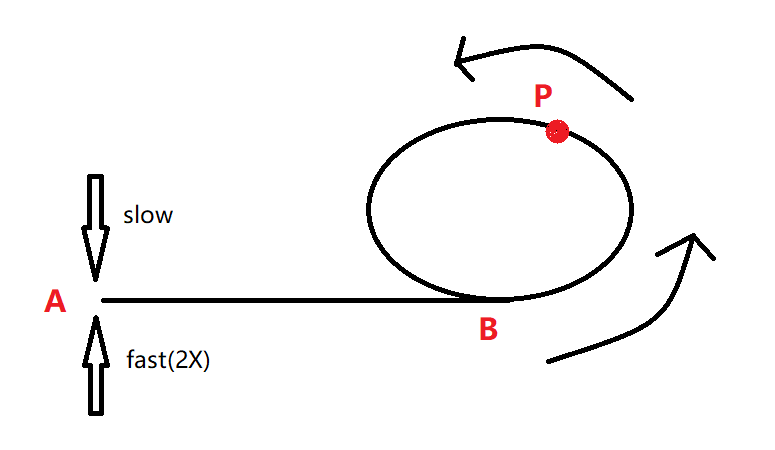
\includegraphics[width=0.7\textwidth]{Fast-and-slow-pointer.png}
	\caption{Fast-and-slow-pointer \label{fig:Fast-and-slow-pointer}}
\end{figure}

代码如下:
\lstinputlisting[language=C++, style=codestyle2]{code03/pollard-rho.cpp}

由于求$GCD$大概会有一个常数,考虑进一步优化。显然如果我们能求得$gcd(ab,N)>1$,那么也是找到了一个因子,只要$a,b$中某一个有$N$的因子即可。
所以我们可以先不急着做$GCD$,而是做一系列的$|t-s|$的连乘,到一定次数再做$GCD$。为了不溢出,我们使连乘的结果$mod\ N$,由欧几里得算法知答案不变。

\lstinputlisting[language=C++, style=codestyle2]{code03/pollard-rho-with-multi.cpp}

pollard-rho算法往往会和miller-rabin同时使用,比如章节题目\ref{prob:pollard}。
其要判断一个数是否是素数,若不是则输出其最大质因子。

代码如下,可作为模板,时间复杂度$O(T*\alpha*(N^{1\over 4}+log^2(N)))$。其中$T$表示数据组数,$\alpha$表示一个不小的常数。

\lstinputlisting[language=C++, style=codestyle2]{code03/luogu-p4718.cpp}

\section{离散对数}

现在我们来思考这样一个问题:

\begin{custom}{问题}
	给定$a,b,m$,求$a^x\equiv b \ (mod \ m)$的解$x$。
\end{custom}

\begin{solution}
	
	我们设$x=A\left \lceil \sqrt{m} \right \rceil -B$,其中$0\le B< \left \lceil \sqrt{m} \right \rceil$, $0< A\le \left \lceil \sqrt{m} \right \rceil+1$,这样化简后的方程是
	$$
	a^{A\left \lceil \sqrt{m} \right \rceil}\equiv b\cdot a^B \quad (mod \ m)
	$$
	由于$A$和$B$值域都是$O(\sqrt{m})$级别的,所以可以先计算右边部分的值,存入$Hash$表,然后从小到大枚举$A$计算左边的值,在$Hash$表中查找。
	(当然,可以这样做的原因是一定存在$a$的逆元)即只要$gcd(a,m)=1$,上面的方法就是有效的。所以当$m$是质数时,用这种方法(Baby Step Giant Step, bsgs)即可。
	
	{\heiti 当$m$不是质数时},我们要求解的是$a^x+km=b$,设$g=gcd(a,m)$,如果$g$不整除$b$,则无解,否则方程两边同除以$g$,得到$\frac{a}{g}a^{x-1}+k\frac{m}{g}=\frac{b}{g}$。
	这样便消去了m的一个因子,得到方程
	$$
	\frac{a}{g}a^{x-1}\equiv \frac{b}{g}\quad (mod \   \frac{m}{g})
	$$
	令${m}'=\frac{m}{g} ,\ b'=\frac{b}{g}(\frac{a}{g})^{-1}$, 得到
	$$
	a^{x'}\equiv b' \quad (mod \ m')
	$$
	于是可以递归,得到的解加1即$x=x'+1$为原方程的解。
	
	{\heiti 但是,进行一次这样的操作,新的方程不一定可以用bsgs求解,所以会进行多次。}
	
	如果中途出现$b'=1$则$x'=0$。
\end{solution}

时间复杂度  $O(\sqrt{m}log\sqrt{m})$,手写二分比unordered\_map会快一点。

\lstinputlisting[language=C++, style=codestyle2]{code03/bsgs.cpp}

注意到代码中有一个技巧,不用把每一步的逆元实际求出来,放到式子左边乘起来就行。
查表时,把初值设置为这个数$*a^{\left \lceil \sqrt{m} \right \rceil}$即可。


\section{原根}
\subsection{幂模$p$与原根}

如果$a$和$p$互素,费马小定理告诉我们,$a^{p-1} \equiv 1\ (mod\ p)$,那么这个指数$p-1$是唯一的使得结果为1的吗?
我们选择一些$a$和$p$来看一下,对于$a=3,p=7$,指数只有为6时才取到1,如表\ref{tab:root}。


\begin{table}[!htbp]
	\centering
	\caption{$a=3,\ p=7$ \label{tab:root}}
	\begin{tabular}{ccc}
		\midrule
		 $3^1\equiv 3(mod\ 7)$  & $3^2\equiv 2(mod\ 7)$ & $3^3\equiv 6(mod\ 7)$ \\
		 $3^4\equiv 4(mod\ 7)$    & $3^5\equiv 5(mod\ 7)$ & $3^6\equiv 1(mod\ 7)$ \\
		 \bottomrule
	\end{tabular}%
\end{table}%

再列多一点,如表\ref{tab:root2},从表中可以看出,似乎有这样的性质:
\begin{itemize}
	\item 对于任何底数,最小指数$e$整除$p-1$;
	\item 总有一些底数,指数需要到$p-1$。
\end{itemize}

\begin{table}[!htbp]
	\centering
	\caption{不同底数对应的最小指数 \label{tab:root2}}
	\begin{tabular}{ccc}
		\toprule
		$p=5$  & $p=7$ & $p=11$ \\
		\midrule
		$1^1\equiv 1(mod\ 5)$  & $1^1\equiv 1(mod\ 7)$ & $1^1\equiv 1(mod\ 11)$ \\
		$2^4\equiv 1(mod\ 5)$    & $2^3\equiv 1(mod\ 7)$ & $2^{10}\equiv 1(mod\ 11)$ \\
		$3^4\equiv 1(mod\ 5)$  & $3^6\equiv 1(mod\ 7)$ & $3^5\equiv 1(mod\ 11)$ \\
		$4^2\equiv 1(mod\ 5)$    & $4^3\equiv 1(mod\ 7)$ & $4^5\equiv 1(mod\ 11)$ \\
	                             & $5^6\equiv 1(mod\ 7)$ & $5^5\equiv 1(mod\ 11)$ \\
		    					& $6^2\equiv 1(mod\ 7)$ & $6^{10}\equiv 1(mod\ 11)$ \\
		  											& & $7^{10}\equiv 1(mod\ 11)$ \\
		   			  								& & $8^{10}\equiv 1(mod\ 11)$ \\
		   			  								& & $9^{5}\equiv 1(mod\ 11)$ \\
		   			  								& & $10^{2}\equiv 1(mod\ 11)$ \\
		\bottomrule
	\end{tabular}%
\end{table}%


为了方便,我们定义$a$模$p$的阶指$e_p(a)=[min\ e\ s.t.\ a^e\equiv 1(mod \ p)]$,其中$a$和$p$互质。另外,规定$e_p(a)\ge 1$,显然$e_p(a)\le p-1$。

\begin{theorem}{次数整除性质}{label}
	设a是不被素数$p$整除的整数,假设$a^n \equiv 1 \ (mod \ p)$,则次数$e_p(a)$整除$n$,特别地$e_p(a)$总整除$p-1$。
\end{theorem}

\begin{proof}
	次数$e_p(a)$的定义告诉我们
	$$
	a^{e_p(a)}\equiv 1 \ (mod \ p)
	$$
	假设$a^n\equiv 1(\ mod \ p)$,
	设$G=gcd(e_p(a),n)$,
	并设$(u,v)$是方程$e_p(a)u-nv=G$的正整数解(可知一定有解)。现在有两种不同的方法计算$a^{e_p(a)u}$:
	\begin{align*}
		a^{e_p(a)u}=(a^{e_p(a)})^u\equiv 1 \ (mod \ p)  \\
		a^{e_p(a)u}=a^{nv+G}\equiv a^G \ (mod \ p)  \\
	\end{align*}

	这表明$a^G\equiv 1 (\ mod \ p)$ ,所以必有$e_p(a)\le G$。
	
	另一方面$G \ | \ e_p(a)$,所以$G=e_p(a)\ ,\ e_p(a)\ | \ n$,证毕。
\end{proof}

{\heiti 现在我们的一个猜想得到了证明,来看另外一个:$e_p(a)=p-1$的底数$a$有什么规律。}

如果a是这样的数,则幂
$$
a^1,\ a^2,\ a^3,\ ...\ ,\ a^{p-2},\ a^{p-1}\quad (\ mod \ p)
$$
{\heiti 必须都是模$p$不同的。}[如果幂不是全不相同,则对某指数$1\le i <j\le p-1$有$a^i\equiv a^j \ (mod \ p)$,由于a,p互质,则有$1\equiv a^{j-i} \ (mod \ p)$,由于$j-i<p-1$,则矛盾]。

{\heiti 这$p-1$个不同的数取遍了$[1,p-1]$。}

{\heiti 这样的数很重要,为了方便,我们称这样的数$g$为模数$p$的原根,即$e_p(g)=p-1$。}

回顾前面的那张表\ref{tab:root2},5的原根是2,3\quad ;\quad 7的原根是3,5\quad ;\quad 11的原根是2,6,7,8。
可见原根可以不止一个,那到底有多少个?所有素数都有原根吗?

\begin{theorem}{原根定理}{label}
每个素数$p$都有原根。更精确地,有恰好$\varphi(p-1)$个原根。
\end{theorem}

神奇!尽管原根定理没有指出求$p$的原根的具体方法,但一旦能求得一个原根,就可以容易得求出其他原根(后面介绍)。求原根的常用方法是从小到大枚举正整数a=2,3,5,6......。{\heiti 因为原根的分布比较广}。(思考为什么没有4)。
为啥没4?因为$4^{\frac{(p-1)}{2}}\equiv 2^{p-1}\equiv 1 \ (mod \ p)$,即4一定不是原根。(可见2的高次幂都不是)

\begin{proof}
	原根定理的证明。
	
	对$1\sim p-1$之间的每个数$a$,$e_p(a) \ | \ (p-1)$ ,所以,对整数$p-1$的每个因子$d$,我们可能会问,有多少个$e_p(a)$等于$d$,由于要用,我们记这个数为$\psi (d),\ 1\le a <p$。 
	$\psi(p-1)$即为模数$p$的原根个数。
	
	设$n$是整除$p-1$的任何数,比如说$p-1=nk$,则可将多项式$X^{p-1}-1$分解成$X^{nk}-1=(X^n)^k-1=(X^n-1)((X^n)^{k-1}+(X^n)^{k-2}+...+(X^n)^2+X^n+1)$
	
	我们数一下这些多项式模$p$有多少个根。
	
	首先,$X^{p-1}-1\equiv 0 \ (mod \ p)$恰好有$p-1$个解,即$[1,p-1]$这些。
	
	另一方面,$(X^n-1)\equiv 0 \ (mod \ p)$至多有$n$个解,且
	$$
	(X^n)^{k-1}+(X^n)^{k-2}+...+(X^n)^2+X^n+1 \equiv 0 \ (mod \ p)
	$$
	至多有$nk-n$个解。
	
	因此我们得到:
	\begin{figure}[htbp]
		\centering
		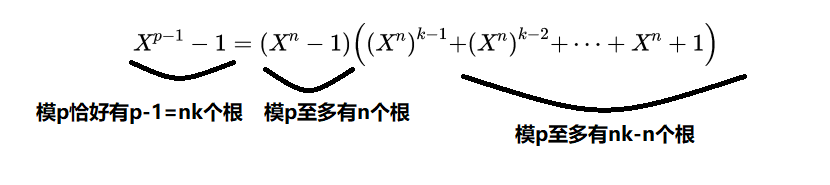
\includegraphics[width=0.7\textwidth]{prime-root.png}
		\caption{根的情况 \label{fig:prime-root}}
	\end{figure}

	上式要成立,$X^n-1$模$p$恰有$n$个根。这就证明了下述重要事实:
	
	{\heiti 如果$n \ | \ p-1$,则同余式$X^n-1\equiv 0 \ (mod \ p)$恰好有$n$个根满足$0\le X<p$。}
	
	现在再用另一种计数方法计数这个同余式的解的个数。如果$X=a$是一个解,则$a^n\equiv 1\ (mod \ p)$,因此$e_p(a)\ | \ n$,即$e_p(a)$对应$n$的一个因子$d$。
	从这个角度,$X^n-1\equiv 0 \ (mod \ p)$解($0\le X<p$)的个数等于:
	$$
		\sum_{d|n}\psi(d)=\psi(d_1)+\psi(d_2)+...+\psi(d_r)
	$$
	
	综合上面两个角度,我们得到一个结论:
	\begin{center}
	{\heiti 若$n$整除$p-1$,则$\sum_{d|n}\psi(d)=n$}
	\end{center}

	
	这个公式和欧拉函数的形式一样!首先,$\varphi(1)=1$,而$\psi(1)=1$,下面证明当$n=q$为素数时,$\psi(n)=\varphi(n)$。
	q的因数是1和q,所以$\psi(q)+\psi(1)=q=\varphi(q)+\varphi(1)$,由于$\psi(1)=\varphi(1)$,则$\psi(q)=\varphi(q)$。$n=q^2$和$n=q_1q_2$也可以类似证明。
	更正式地,可以给出归纳证明,这里不展示了。
	
	证毕。
\end{proof}

{\heiti 综上,我们已证明对整除$p-1$的每个整数$n$,恰好有$\varphi(n)$个底数$a$使得$e_p(a)=n$,取$n=p-1$,则$\varphi(p-1)$为原根个数。显然,每个素数至少有一个原根。}

\vbox{}

{\heiti 求原根,时间复杂度: 对于单个$p$,$O(\sqrt{p} + T*logn*logn)$   ;对于区间问题,可以做到$O(nlogn + \frac{n}{logn}*T*logn*logn)$,其中$T$表示平均意义下每个素数最小原根。
除以$logn$是因为素数的分布。}
\lstinputlisting[language=C++, style=codestyle2]{code03/primitive-root.cpp}

\subsection{原根与指标}
我们大概知道原根是啥了,那指标是什么呢?对于模数13,2是它的原根,那么$2^x\ mod \ 13$会取遍$[1,12]$里所有的数,$x\in [1,12]$。
{\heiti 而指标函数$I$就是从余数到指数的双射函数。}比如$2^4\equiv 3\ (mod\ 13)$,则$I(3) = 4$。



\begin{theorem}{指标法则}{label}
	指标满足下述法则:
		\begin{itemize}
			\item $I(ab)\equiv I(a)+I(b) \quad (mod \ p-1)$ \quad  乘积法则
			\item $I(a^k)\equiv k*I(a)  \quad (mod \ p-1)$ \quad  幂法则
		\end{itemize}
\end{theorem}

\begin{note}
	模数是$p-1$。
\end{note}

\begin{proof}
	 $g^{I(ab)}\equiv ab\equiv g^{I(a)}g^{I(b)}\equiv g^{I(a)+I(b)}\quad (mod \ p)$
	
	这意味着$g^{I(ab)-I(a)-I(b)}\equiv 1\ (mod \ p)$,又$g$是原根,则$I(ab)-I(a)-I(b)$是$p-1$的倍数。
	
	所以乘积法则得证。幂法则同理。
\end{proof}

\vbox{}

利用指标这个工具,可以方便地解一些高次同余方程。

\begin{custom}{问题}
求同余式$3x^{30}\equiv 4\ (mod \ 37)$。
\end{custom}

\begin{solution}
	使用乘积法则和幂法则:
$$
\begin{aligned} I\left(3 x^{30}\right) &=I(4) \\ I(3)+30 I(x) & \equiv I(4)(\bmod 36) \\ 26+30 I(x) &\equiv2(\bmod 36) \\ 30 I(x) & \equiv-24\equiv12(\bmod 36) \end{aligned}
$$
对于最后一个式子,是一个同余方程,由于$gcd(30,36)=6\ |\ 12$,则其有解,且有6个不同余解。
我们求得
$$
I(x)\equiv 4,\ 10,\ 16,\ 22,\ 28,\ 34 \quad (mod \ 36)
$$
再查双射表得到对应的值,有6个解$16,\ 25,\ 9,\ 21,\ 12,\ 28$。
\end{solution}

可以看到指标法的优点在于将{\heiti 幂运算转为乘法,将乘法转为加法}。这一点和对数函数很像:
$$
\begin{aligned} \log (a b) &=\log (a)+\log (b) \\ \log \left(a^{k}\right) &=k \log (a) \end{aligned}
$$

类似这一题的同余式称为剩余问题,下一章我们就来研究一下。这一章就到这。


\vbox{}

\vbox{}

\begin{problemset}
	\item \href{http://poj.org/problem?id=2891}{Strange Way to Express Integers \quad POJ2891 \quad 同余方程组,模数不一定互质}  
	\item \href{https://cn.vjudge.net/problem/Gym-101550E#}{Exponial \quad 欧拉降幂}
	\item \href{http://acm.hdu.edu.cn/showproblem.php?pid=4910}{Problem about GCD \quad 威尔逊定理的应用}
	\item \href{https://vjudge.net/problem/HDU-5391}{Zball in Tina Town \quad 威尔逊定理 \quad 素性测试}
	\item \href{https://www.luogu.org/problem/P4718}{【模板】Pollard-Rho算法 \quad 素性测试 \quad Pollard\_Rho质因数分解 \label{prob:pollard}}
	\item \href{https://www.spoj.com/problems/MOD/}{MOD - Power Modulo Inverted \quad 离散对数}
	\item 对任何正整数$k$,求$1^k+2^k+3^k+...+(p-1)^k\ (mod\ p)$的值。 \  ans:0 \href{https://math.stackexchange.com/questions/1049420/for-any-positive-number-k-find-the-value-of-1k-2k-3k-p-1kmod?r=SearchResults#}{solution}
	\item (2017四川省赛K.2017)给你$n$(不超过200w)个数,和一个数$r$,问你有多少种方案,使得你取出某个子集,能够让它们的乘积$mod \ 2017$等于$r$。由于
	方案数众多,最后只需要输出答案的奇偶性即可。\href{https://www.cnblogs.com/autsky-jadek/p/7496328.html}{\quad 原根}
\end{problemset}


\chapter{常见问题集}

\begin{custom}{问题}
有没有办法章节用“第一章,第一节,(一)”这种?
\end{custom}

\begin{solution}
你可以修改模板中对于章节的设置,利用 ctex 宏集的 \lstinline{\zhnumber} 命令可以把计数器的数字形式转为中文。
\end{solution}


\begin{custom}{问题}
3.07 版本的 cls 的 natbib 加了numbers 编译完了没变化,群主设置了不可更改了?
\end{custom}

\begin{solution}
3.07 中在 \lstinline{gbt7714} 宏包使用时,加入了 \lstinline{authoryear} 选项,这个使得 \lstinline{natbib} 设置了 \lstinline{numbers} 也无法生效。3.08 和 3.09 版本中,模板新增加了 \lstinline{numbers} 、\lstinline{super} 和 \lstinline{authoryear} 文献选项,你可以参考前文设置说明。
\end{solution}

\begin{custom}{问题}
大佬,我想把正文字体改为亮色,背景色改为黑灰色。
\end{custom}

\begin{solution}
页面颜色可以使用 \lstinline{\pagecolor} 命令设置,文本命令可以参考\href{https://tex.stackexchange.com/questions/278544/xcolor-what-is-the-equivalent-of-default-text-color}{这里}进行设置。
\end{solution}

\begin{custom}{问题}
\lstinline[breaklines]{Package ctex Error: CTeX fontset `Mac' is unavailable.}
\end{custom}

\begin{solution}
在 Mac 系统下,中文编译请使用 \lstinline{XeLaTeX}。
\end{solution}

\begin{custom}{问题}
\lstinline{! LaTeX Error: Unknown option `scheme=plain' for package `ctex'.}
\end{custom}

\begin{solution}
你用的 C\TeX{} 套装吧?这个里面的 \lstinline{ctex} 宏包已经是已经是 10 年前的了,与本模板使用的 \lstinline{ctex} 宏集有很大区别。不建议 C\TeX{} 套装了,请卸载并安装 \TeX{} Live 2019。
\end{solution}

\begin{custom}{问题}
我该使用什么版本?
\end{custom}

\begin{solution}
请务必使用\href{https://github.com/ElegantLaTeX/ElegantBook/releases}{最新正式发行版},发行版间不定期可能会有更新(修复 bug 或者改进之类),如果你在使用过程中没有遇到问题,不需要每次更新\href{https://github.com/ElegantLaTeX/ElegantBook/archive/master.zip}{最新版},但是在发行版更新之后,请尽可能使用最新版(发行版)!最新发行版可以在 Github 或者 \TeX{} Live 2019 内获取。
\end{solution}


\begin{custom}{问题}
我该使用什么编辑器?
\end{custom}

\begin{solution}
你可以使用 \TeX{} Live 2019 自带的编辑器 \TeX{}works 或者使用 \TeX{}studio,\TeX works 的自动补全,你可以参考我们的总结 \href{https://github.com/EthanDeng/texworks-autocomplete}{\TeX works 自动补全}。推荐使用 \TeX{} Live 2019 + \TeX Studio。我自己用 VS Code 和 Sublime Text,相关的配置说明,请参考 \href{https://github.com/EthanDeng/vscode-latex}{\LaTeX{} 编译环境配置:Visual Studio Code 配置简介} 和 \href{https://github.com/EthanDeng/sublime-text-latex}{Sublime Text 搭建 \LaTeX{} 编写环境}。
\end{solution}


\begin{custom}{问题}
您好,我们想用您的 ElegantBook 模板写一本书。关于机器学习的教材,希望获得您的授权,谢谢您的宝贵时间。
\end{custom}

\begin{solution}
模板的使用修改都是自由的,你们声明模板来源以及模板地址(github 地址)即可,其他未尽事宜按照开源协议 LPPL-1.3c。做好之后,如果方便的话,可以给我们一个链接,我把你们的教材放在 ElegantLaTeX 用户作品集里。
\end{solution}

\begin{custom}{问题}
我想要原来的封面!
\end{custom}

\begin{solution}
我们计划在未来版本加入封面选择,让用户可以选择旧版封面。
\end{solution}

\begin{custom}{问题}
我想修改中文字体!
\end{custom}

\begin{solution}
首先,我们{\heiti 强烈建议你不要去修改字体}!如果你一定坚持修改字体,请在 \lstinline{newtxtext} 宏包加载前加入中文字体设置(\lstinline{xeCJK} 宏包)。

如果你选择自定义字体,请设置好 \lstinline{\kaishu},\lstinline{\heiti} 等命令,否则会报错。如果你看不懂我现在说的,请停止你的字体自定义行为。
\end{solution}

\begin{custom}{问题}
请问交叉引用是什么?
\end{custom}

\begin{solution}
本群和本模板适合有一定 \LaTeX{} 基础的用户使用,新手请先学习 \LaTeX{} 的基础,理解各种概念,否则你将寸步难行。
\end{solution}

\begin{custom}{问题}
定义等环境中无法使用加粗命令么?
\end{custom}

\begin{solution}
是这样的,默认中文并没加粗命令,如果你想在定义等环境中使用加粗命令,请使用 \lstinline{\heiti} 等字体命令,而不要使用 \lstinline{\textbf}。或者,你可以将 \lstinline{\textbf} 重新定义为 \lstinline{\heiti}。英文模式不存在这个问题。
\end{solution}

\begin{custom}{问题}
代码高亮环境能用其他语言吗?
\end{custom}

\begin{solution}
可以的,ElegantBook 模板用的是 \lstinline{listings} 宏包,你可以在环境(\lstinline{lstlisting})之后加上语言(比如 Python 使用 \lstinline{language=Python} 选项),全局语言修改请使用 \lstinline{\lstset} 命令,更多信息请参考宏包文档。
\end{solution}


\begin{custom}{问题}
群主,什么时候出 Beamer 的模板(主题),ElegantSlide 或者 ElegantBeamer?
\end{custom}

\begin{solution}
这个问题问的人比较多,我这里给个明确的答案。由于 Beamer 中有一个很优秀的主题 \href{https://github.com/matze/mtheme}{Metropolis}。我觉得在我们找到非常好的创意之前不会发布正式的 Beamer 主题,如果你非常希望得到 Elegant\LaTeX{} “官方”的主题,请在用户 QQ 群内下载我们测试主题 PreElegantSlide(未来不一定按照这个制作)。正式版制作计划在 2020 年之后。
\end{solution}


\nocite{*} 

\bibliography{reference}
\include{05indefiniteequation}
\chapter{其他}
\begin{introduction}[本章内容提要]
	\item 斐波那契循环节
\end{introduction}

斐波那契循环节

\appendix

\chapter{常用的表}


\section{梅森素数表}


\section{卡米歇尔数}
1 561

2 1105

3 1729

4 2465

5 2821

6 6601

7 8911

8 10585

9 15841

10 29341

11 41041

12 46657

13 52633

14 62745

15 63973

16 75361

17 101101

18 115921

19 126217

20 162401

21 172081

22 188461

23 252601

24 278545

25 294409

\section{常见的素数及其原根}

\begin{table}[!htbp]
\centering
\caption{常见的素数及其原根 \label{tab:ntt-primes}}
\begin{tabular}{|c|c|c|c|}
\hline
$p=k*2^m + 1$         & $k$   & $m$  & $groot$ \\ \hline
3                   & 1   & 1  & 2     \\ \hline
5                   & 1   & 2  & 2     \\ \hline
17                  & 1   & 4  & 3     \\ \hline
97                  & 3   & 5  & 5     \\ \hline
193                 & 3   & 6  & 5     \\ \hline
257                 & 1   & 8  & 3     \\ \hline
7681                & 15  & 9  & 17    \\ \hline
12289               & 3   & 12 & 11    \\ \hline
40961               & 5   & 13 & 3     \\ \hline
65537               & 1   & 16 & 3     \\ \hline
786433              & 3   & 18 & 10    \\ \hline
5767169             & 11  & 19 & 3     \\ \hline
7340033             & 7   & 20 & 3     \\ \hline
23068673            & 11  & 21 & 3     \\ \hline
104857601           & 25  & 22 & 3     \\ \hline
167772161           & 5   & 25 & 3     \\ \hline
469762049           & 7   & 26 & 3     \\ \hline
{ \color{red}998244353}           & 119 & 23 & 3     \\ \hline
{\color{red}1004535809}          & 479 & 21 & 3     \\ \hline
2013265921          & 15  & 27 & 31    \\ \hline
{\color{red}2281701377}          & 17  & 27 & 3     \\ \hline
3221225473          & 3   & 30 & 5     \\ \hline
75161927681         & 35  & 31 & 3     \\ \hline
77309411329         & 9   & 33 & 7     \\ \hline
206158430209        & 3   & 36 & 22    \\ \hline
2061584302081       & 15  & 37 & 7     \\ \hline
2748779069441       & 5   & 39 & 3     \\ \hline
6597069766657       & 3   & 41 & 5     \\ \hline
39582418599937      & 9   & 42 & 5     \\ \hline
79164837199873      & 9   & 43 & 5     \\ \hline
263882790666241     & 15  & 44 & 7     \\ \hline
1231453023109121    & 35  & 45 & 3     \\ \hline
1337006139375617    & 19  & 46 & 3     \\ \hline
3799912185593857    & 27  & 47 & 5     \\ \hline
4222124650659841    & 15  & 48 & 19    \\ \hline
7881299347898369    & 7   & 50 & 6     \\ \hline
31525197391593473   & 7   & 52 & 3     \\ \hline
180143985094819841  & 5   & 55 & 6     \\ \hline
1945555039024054273 & 27  & 56 & 5     \\ \hline
4179340454199820289 & 29  & 57 & 3     \\ \hline
\end{tabular}
\end{table}
\chapter{最小示例}

\begin{lstlisting}
\documentclass[lang=cn,11pt]{elegantbook}
% title info
\title{Title}
\subtitle{Subtitle is here}
% bio info
\author{Your Name}
\institute{XXX University}
\date{\today}
% extra info
\version{1.00}
\extrainfo{Victory won\rq t come to us unless we go to it. --- M. Moore}
\logo{logo.png}
\cover{cover.jpg}

\begin{document}

\maketitle
\tableofcontents
\mainmatter
\hypersetup{pageanchor=true}
% add preface chapter here if needed
\chapter{Example Chapter Title}
The content of chapter one.

\bibliography{reference}

\end{document}
\end{lstlisting}



\end{document}
